\documentclass{standalone}
\usepackage{tikz}

\begin{document}
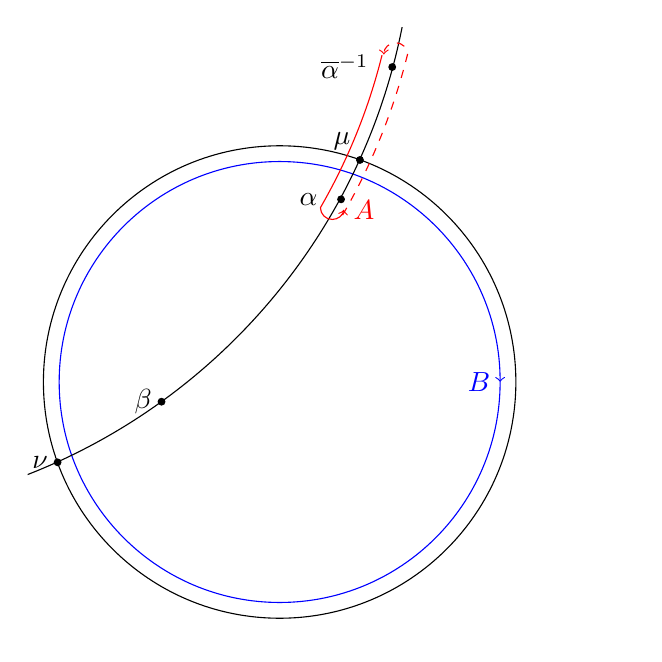
\begin{tikzpicture}
\clip (-3.2,-3.2) rectangle (4.5,4.5);

% unit circle
\draw (0,0) circle [radius=3];
% blue B period just inside unit circle
\draw[color=blue,<-] (2.8,0) arc (0:360:2.8) node[left, color=blue]{$B$};

% branch point circle
\draw[color=black] (-6,6) circle [radius=7.7];
% red A period, in two halves
\draw[color=red,dashed,->] (0.80,2.12) arc (330:346:7.9) arc (0:180:0.15);
\draw[color=red,->] (1.3,4.15)  arc (346:330:7.5) arc (180:350:0.15) node[right, color=red]{$A$};

% points
\fill (1.02,2.82) circle (0.05) node[above left, color=black]{$\mu$};
\fill (0.78,2.32) circle (0.05) node[left=5pt, color=black]{$\alpha$};
\fill (1.43,4) circle (0.05) node[left=5pt, color=black]{$\overline{\alpha}^{-1}$};
\fill (-1.5,-0.25) circle (0.05) node[left, color=black]{$\beta$};
\fill (-2.82,-1.02) circle (0.05) node[left, color=black]{$\nu$};

\end{tikzpicture}
\end{document}
